\documentclass{standalone}
\usepackage{tikz}

\begin{document}
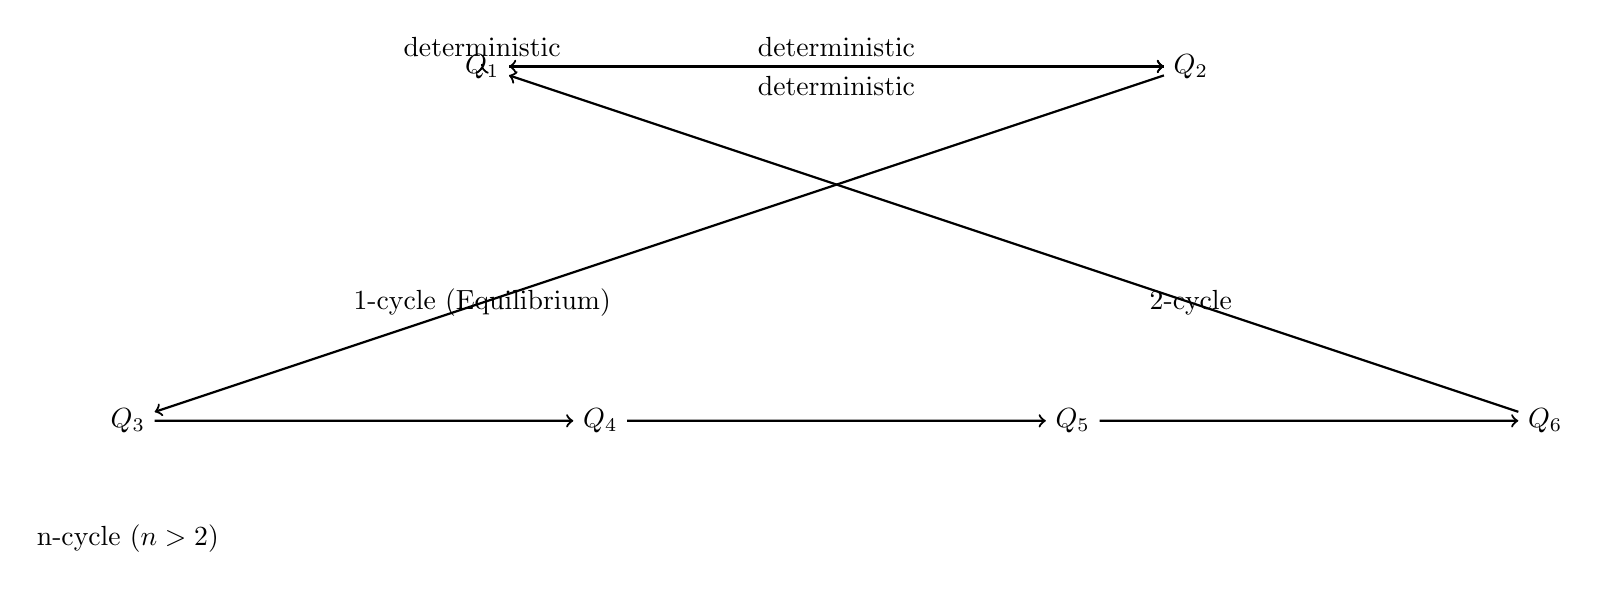
\begin{tikzpicture}[scale=1.5]

% Define nodes for states
\node (state1) at (-3,0) {$Q_1$};
\node (state2) at (3,0) {$Q_2$};

% Draw arrows for 1-cycle (equilibrium)
\draw[->, thick] (state1) -- node[midway, above] {deterministic} (state1);

% Draw arrows for 2-cycle
\draw[->, thick] (state1) -- node[midway, below] {deterministic} (state2);
\draw[->, thick] (state2) -- node[midway, above] {deterministic} (state1);

% Nodes for n-cycle (n > 2)
\node (state3) at (-6,-3) {$Q_3$};
\node (state4) at (-2,-3) {$Q_4$};
\node (state5) at (2,-3) {$Q_5$};
\node (state6) at (6,-3) {$Q_6$};

% Draw arrows for n-cycle
\foreach \i in {1,...,5} {
    \draw[->, thick] (state\i) -- (state\the\numexpr\i+1\relax);
}
\draw[->, thick] (state6) -- (state1);

% Add labels
\node at (-3,-2) {1-cycle (Equilibrium)};
\node at (3,-2) {2-cycle};
\node at (-6,-4) {n-cycle ($n > 2$)};
\end{tikzpicture}
\end{document}